\pdfminorversion=4
\documentclass[aspectratio=169]{beamer}

\mode<presentation>
{
  \usetheme{default}
  \usecolortheme{default}
  \usefonttheme{default}
  \setbeamertemplate{navigation symbols}{}
  \setbeamertemplate{caption}[numbered]
  \setbeamertemplate{footline}[frame number]  % or "page number"
  \setbeamercolor{frametitle}{fg=white}
  \setbeamercolor{footline}{fg=black}
} 

\usepackage[english]{babel}
\usepackage[utf8x]{inputenc}
\usepackage{tikz}
\usepackage{courier}
\usepackage{array}
\usepackage{bold-extra}
\usepackage{minted}
\usepackage[thicklines]{cancel}
\usepackage{fancyvrb}

\xdefinecolor{dianablue}{rgb}{0.18,0.24,0.31}
\xdefinecolor{darkblue}{rgb}{0.1,0.1,0.7}
\xdefinecolor{darkgreen}{rgb}{0,0.5,0}
\xdefinecolor{darkgrey}{rgb}{0.35,0.35,0.35}
\xdefinecolor{darkorange}{rgb}{0.8,0.5,0}
\xdefinecolor{darkred}{rgb}{0.7,0,0}
\definecolor{darkgreen}{rgb}{0,0.6,0}
\definecolor{mauve}{rgb}{0.58,0,0.82}

\title[2018-11-07-hsf-hep-in-numpy]{HEP analysis in the Numpy ecosystem}
\author{Jim Pivarski}
\institute{Princeton University -- DIANA-HEP}
\date{November 7, 2018}

\usetikzlibrary{shapes.callouts}

\begin{document}

\logo{\pgfputat{\pgfxy(0.11, 7.4)}{\pgfbox[right,base]{\tikz{\filldraw[fill=dianablue, draw=none] (0 cm, 0 cm) rectangle (50 cm, 1 cm);}\mbox{\hspace{-8 cm}
\includegraphics[height=1 cm]{princeton-logo-long.png}
\includegraphics[height=1 cm]{diana-hep-logo-long.png}}}}}

\begin{frame}
  \titlepage
\end{frame}

\logo{\pgfputat{\pgfxy(0.11, 7.4)}{\pgfbox[right,base]{\tikz{\filldraw[fill=dianablue, draw=none] (0 cm, 0 cm) rectangle (50 cm, 1 cm);}\mbox{\hspace{-8 cm}
\includegraphics[height=1 cm]{princeton-logo.png}
\includegraphics[height=1 cm]{diana-hep-logo.png}}}}}

% Uncomment these lines for an automatically generated outline.
%\begin{frame}{Outline}
%  \tableofcontents
%\end{frame}

% START START START START START START START START START START START START START

\begin{frame}{In case we need a ``Motivations'' section}
\vspace{0.25 cm}
\begin{center}
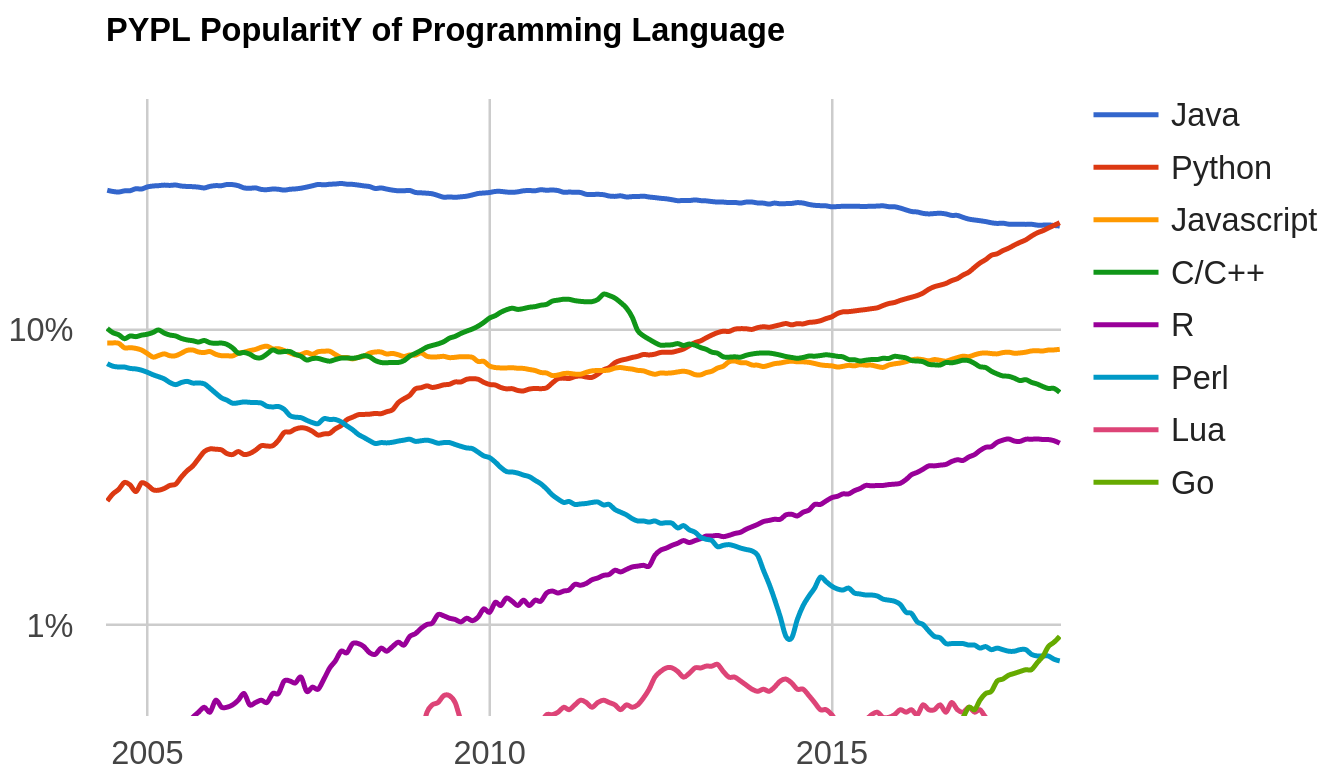
\includegraphics[width=0.8\linewidth]{pypl-popularity.png}
\end{center}
\textcolor{blue}{\scriptsize\url{http://pypl.github.io/PYPL.html}}
\end{frame}

\begin{frame}{In case we need a ``Motivations'' section}
\vspace{0.5 cm}
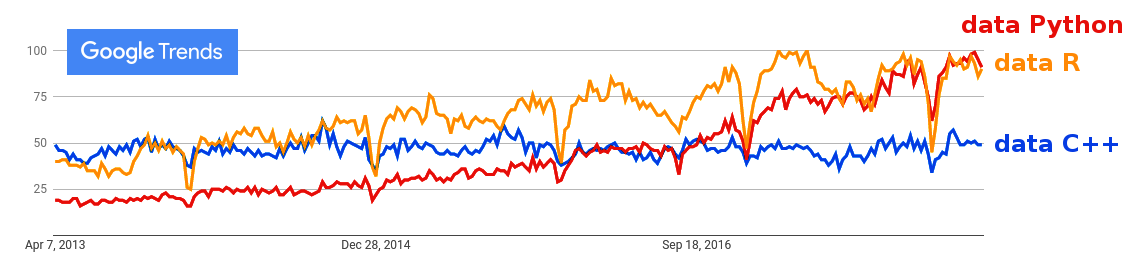
\includegraphics[width=\linewidth]{python-r-cpp-googletrends-data.png}

\vspace{1 cm}
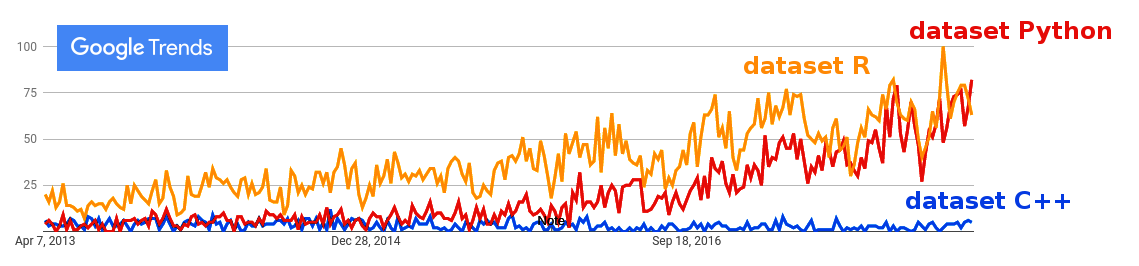
\includegraphics[width=\linewidth]{python-r-cpp-googletrends-dataset.png}
\end{frame}

\begin{frame}{In case we need a ``Motivations'' section}
\vspace{0.5 cm}
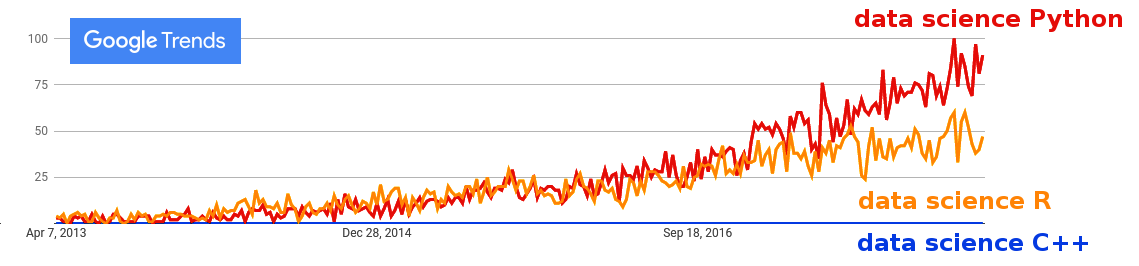
\includegraphics[width=\linewidth]{python-r-cpp-googletrends-datascience.png}

\vspace{1 cm}
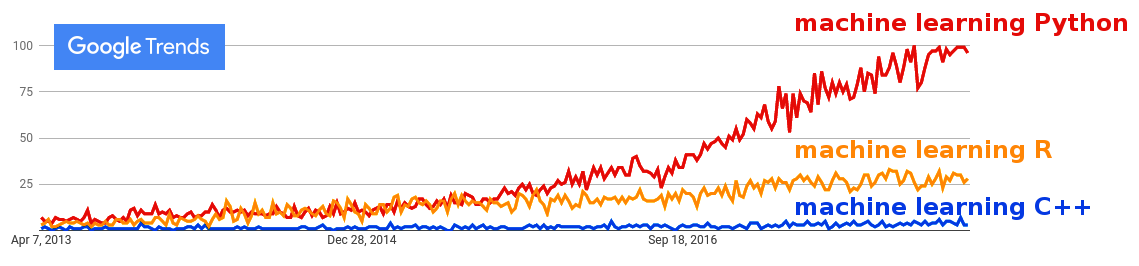
\includegraphics[width=\linewidth]{python-r-cpp-googletrends-machinelearning.png}
\end{frame}

\begin{frame}{In case we need a ``Motivations'' section}
\vspace{0.5 cm}
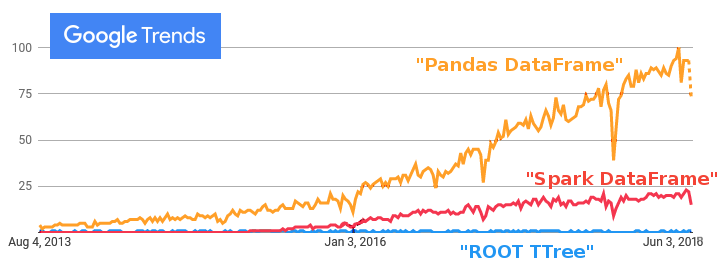
\includegraphics[width=\linewidth]{root-spark-pandas-google-trends.png}
\end{frame}

\begin{frame}{Stealing from Jake VanderPlas's {\it Unexpected Effectiveness} talk}
\vspace{0.25 cm}
\begin{columns}[b]
\column{0.75\linewidth}
\only<1>{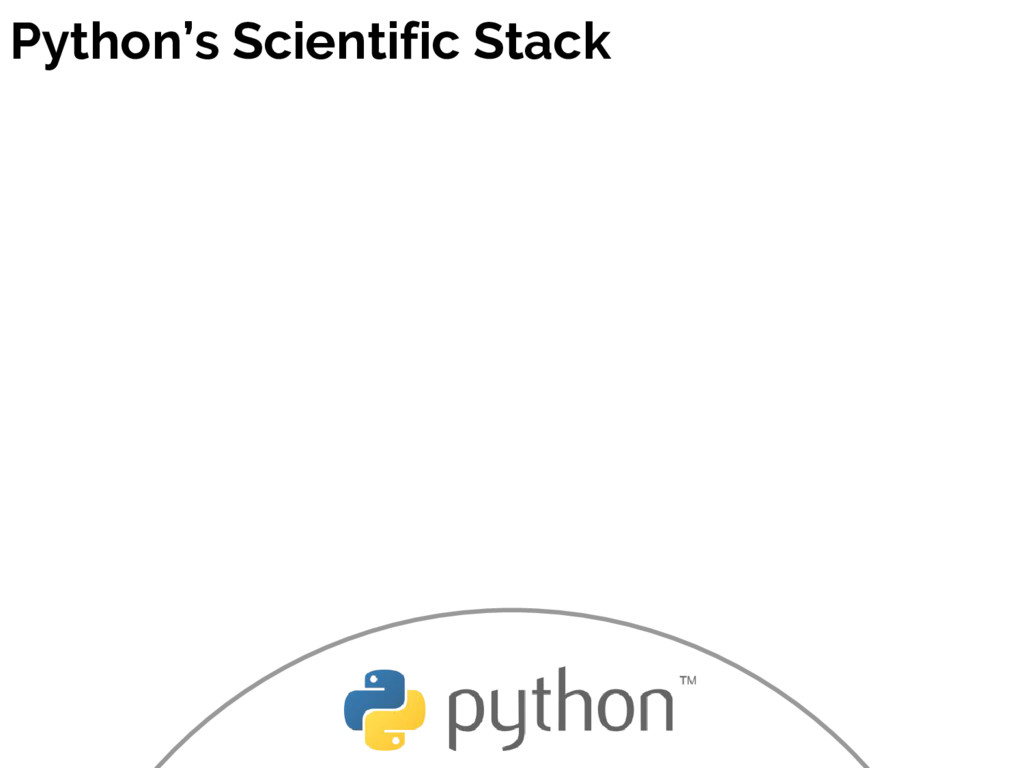
\includegraphics[height=7.8 cm]{shells-1.png}}
\only<2>{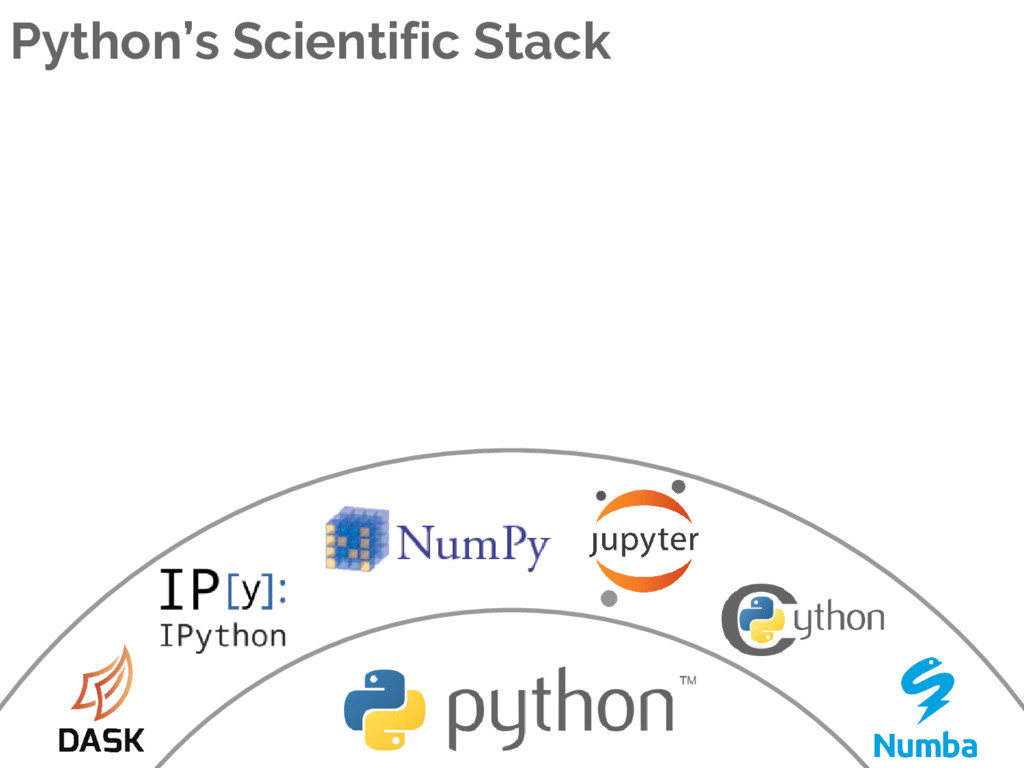
\includegraphics[height=7.8 cm]{shells-2.png}}
\only<3>{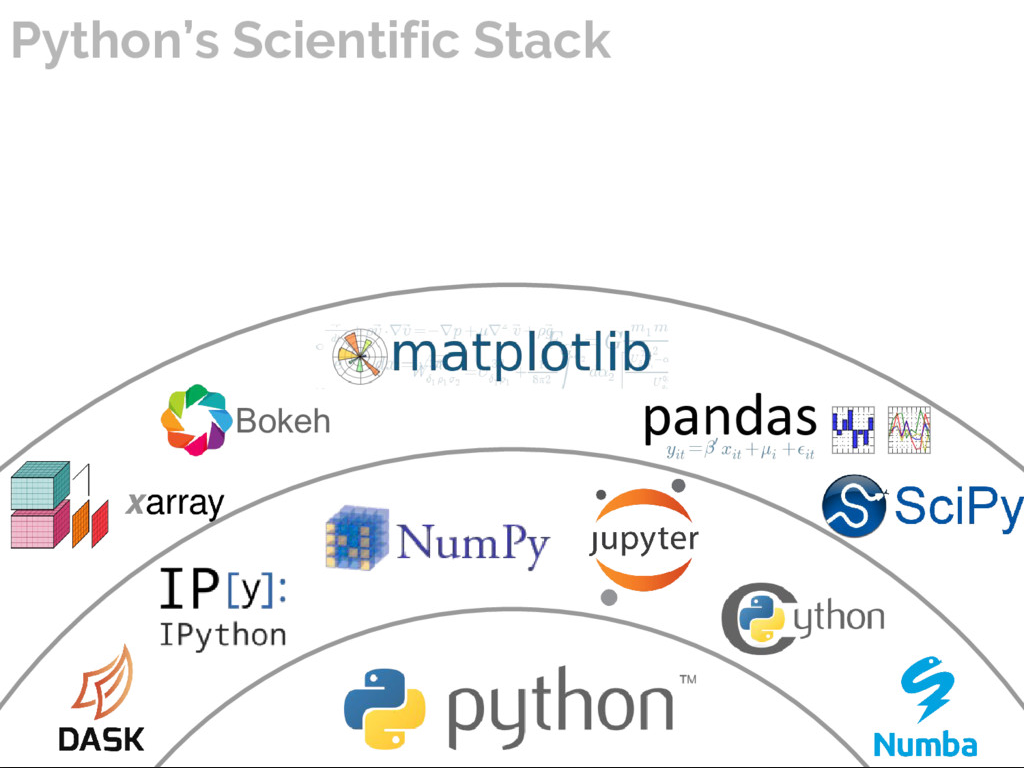
\includegraphics[height=7.8 cm]{shells-3.png}}
\only<4>{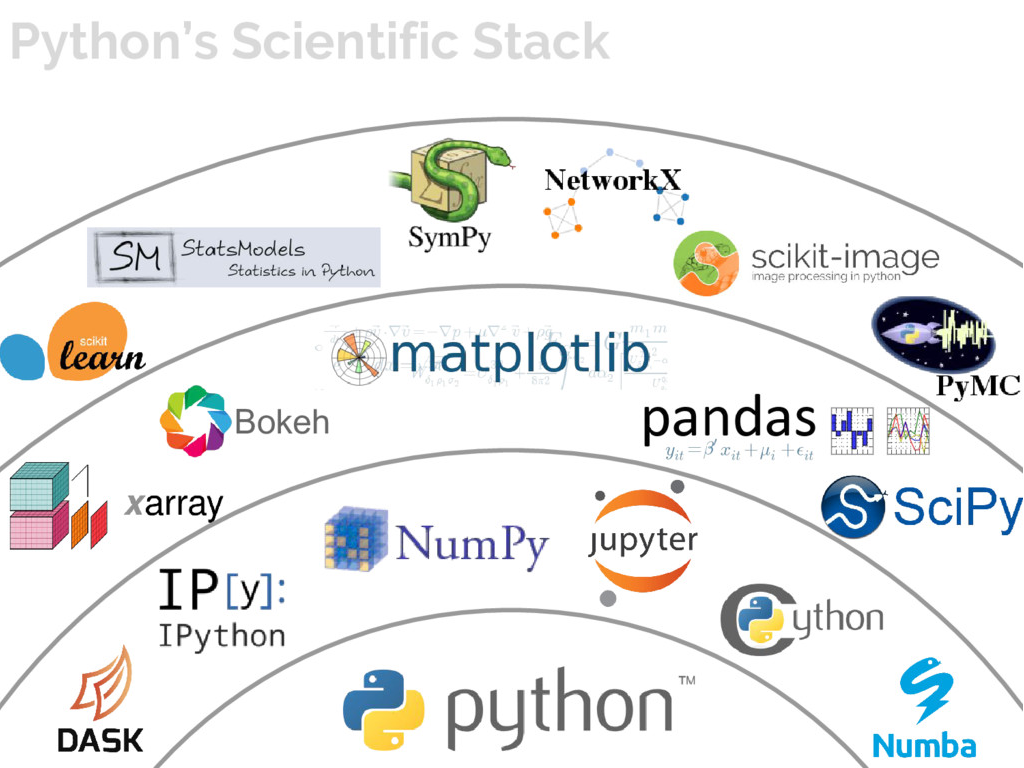
\includegraphics[height=7.8 cm]{shells-4.png}}
\only<5>{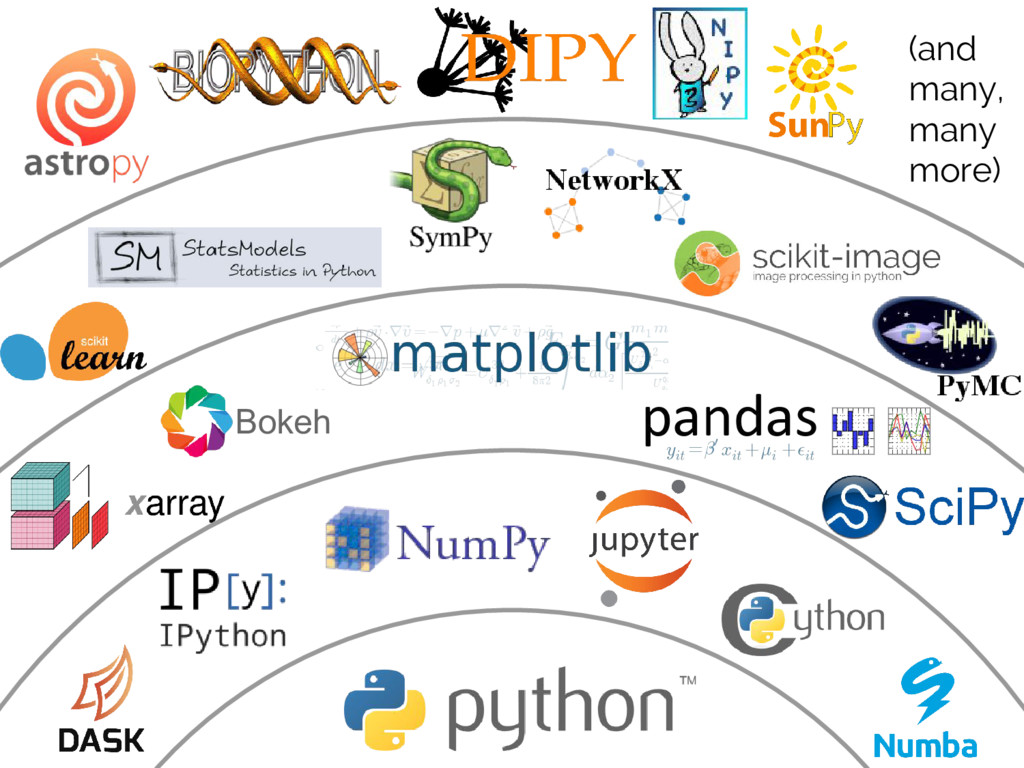
\includegraphics[height=7.8 cm]{shells-5.png}\vspace{0.5 cm}}

\column{0.25\linewidth}

\includegraphics[width=\linewidth]{unreasonable-effectiveness.png}
\vspace{5.3 cm}
\end{columns}
\end{frame}

\begin{frame}{The other sciences are doing it, so why can't I?}
\vspace{0.3 cm}
\begin{columns}[b]
\column{0.59\linewidth}
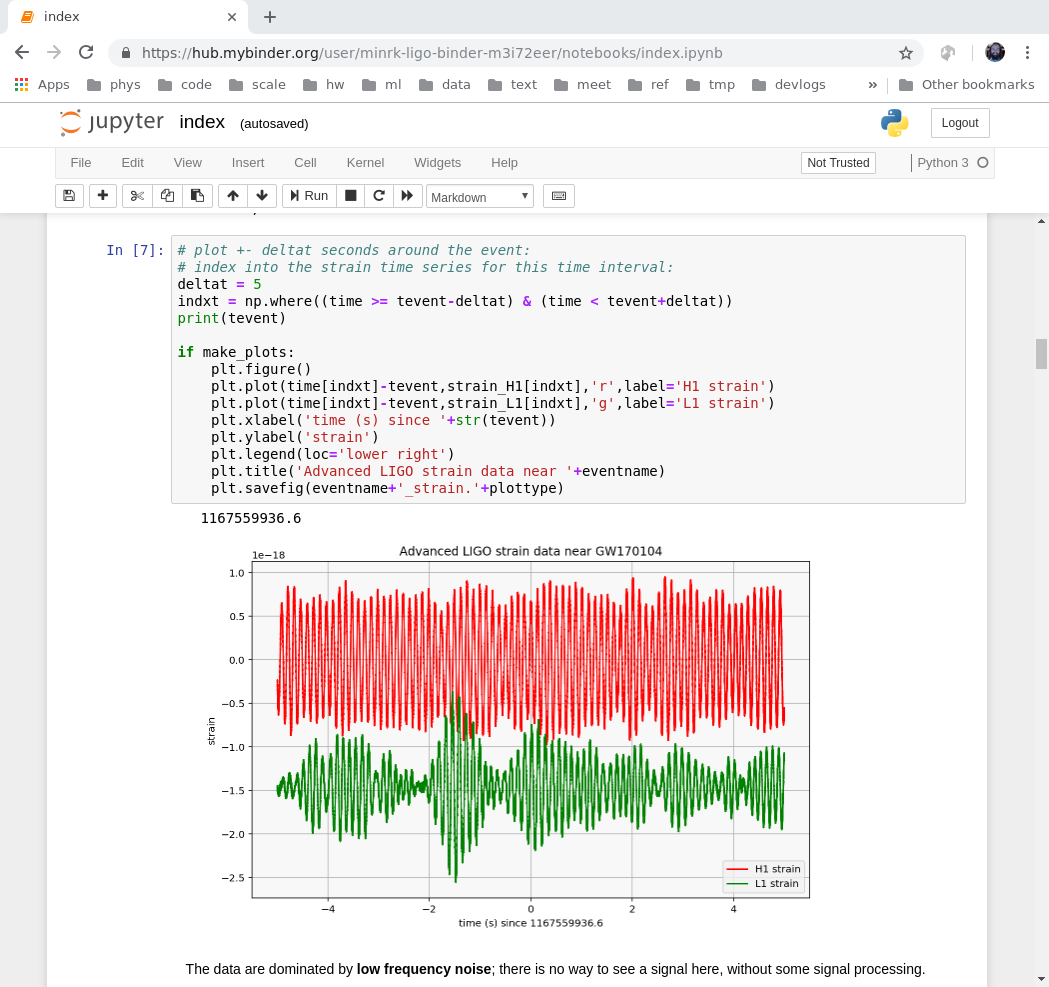
\includegraphics[width=\linewidth]{lsst-notebook.png}

\column{0.41\linewidth}
\begin{itemize}\setlength{\itemsep}{0.5 cm}
\item LIGO full analysis in \\ Numpy $+$ Jupyter $+$ Binder \\ $\to$ you can run all the signal processing yourself without downloading anything.
\item LSST is adopting Python $+$ Jupyter as the general astronomer's interface.
\item XENON-nT is doing their full stack in Python $+$ Numpy.
\item (easy to find examples\ldots)
\end{itemize}

\vspace{0.75 cm}
\end{columns}
\end{frame}

\begin{frame}{Why not indeed?}
\vspace{0.5 cm}
Numpy allowed Python to fill a niche occupied by MATLAB and R: transforming, filtering, signal processing, and machine learning on GB's of rectangular array data.

\vspace{0.75 cm}
\begin{columns}[t]
\column{0.1\linewidth}

\column{0.3\linewidth}
\textcolor{darkgreen}{\bf Python for loops are expressive but not fast.}

\vspace{0.25 cm}
Good for small, complex processing that needs a fully nested object model.

\column{0.3\linewidth}
\textcolor{darkorange}{\bf Numpy arrays are \\ fast but not expressive.}

\vspace{0.25 cm}
Good for biggish, more regular processing (including ML).

\column{0.1\linewidth}
\end{columns}

\vspace{0.75 cm}
Most astronomy, data science, etc.\ fits one of these cases.
\end{frame}

\begin{frame}{Three surmountable challenges}
\large
\vspace{0.5 cm}
\begin{center}
\begin{minipage}{0.75\linewidth}
\begin{enumerate}\setlength{\itemsep}{1 cm}
\item HEP software stacks and conventions were developed {\it before} the Numpy ecosystem and have to be retrofitted to communicate easily.

\item HEP analysis relies heavily on nested data: each event may have a different number of particles.

\item HEP analysis must be performed on TB of ntuples or PB of centrally produced data with thousands of users hitting the same system/files.
\end{enumerate}
\end{minipage}\mbox{\hspace{1 cm}}
\end{center}
\end{frame}

\begin{frame}{}
\LARGE
\vspace{1 cm}
\begin{center}
\textcolor{darkblue}{1. HEP software $\leftrightarrow$ Numpy}
\end{center}
\end{frame}

\begin{frame}{An active area for a long time and now accelerating}
\vspace{0.5 cm}
\begin{itemize}\setlength{\itemsep}{0.5 cm}
\item The PyROOT project started in 2003, just before release 2.3 of \raisebox{-0.2\height}{
\includegraphics[height=\baselineskip]{old-python-logo.png}}.

Every C++ class/function is accessible in Python, at a performance price.

\item Many small HEP packages address specific access issues:

\vspace{0.05 cm}
\begin{itemize}\setlength{\itemsep}{0.05 cm}
\item PyMinuit: extracted from my HEP analysis and open sourced in 2005
\item iminuit: modern version, used in astronomy
\item rootpy: more ``Pythonic'' interface overlaid on PyROOT
\item root\_numpy: faster bindings compiled into C++
\item {\bf 81} packages matching ``HEP'' in PyPI; {\bf 247} with ``HEP'' and Python in GitHub\ldots
\end{itemize}

\item The ROOT team is actively adding ``Pythonizations'' to PyROOT for a more Pythonic interface and also direct-to-Numpy access.

\vspace{0.1 cm}
\begin{itemize}\setlength{\itemsep}{0.1 cm}
\item {\tt\small ttree.AsMatrix()}: access TTree data in Python as Numpy
\item RDataFrame sources and sinks to include Numpy arrays and Arrow
\end{itemize}
\end{itemize}
\end{frame}

\begin{frame}{Scikit-HEP}
\large
\vspace{0.2 cm}
\begin{columns}
\column{2.5 cm}
\hfill 
\includegraphics[width=0.8\linewidth]{skhep-logo.pdf}

\column{0.8\linewidth}
{\bf Scikit-HEP:} an attempt to build community around a suite of interoperating Pythonic HEP libraries, like PyData or AstroPy.
\end{columns}

\begin{columns}
\column{2.5 cm}
\hfill 
\includegraphics[width=0.8\linewidth]{uproot-logo.pdf}

\column{0.8\linewidth}
{\bf uproot:} reader and writer of the ROOT file format in Python.
\end{columns}

\vspace{0.1 cm}
\begin{columns}
\column{2.5 cm}

\includegraphics[width=\linewidth]{awkward-logo.pdf}

\column{0.8\linewidth}
{\bf awkward-array:} extensions of array programming idioms to non-rectangular and deeply nested data.
\end{columns}

\vspace{0.3 cm}
\begin{columns}
\column{2.5 cm}
\hfill 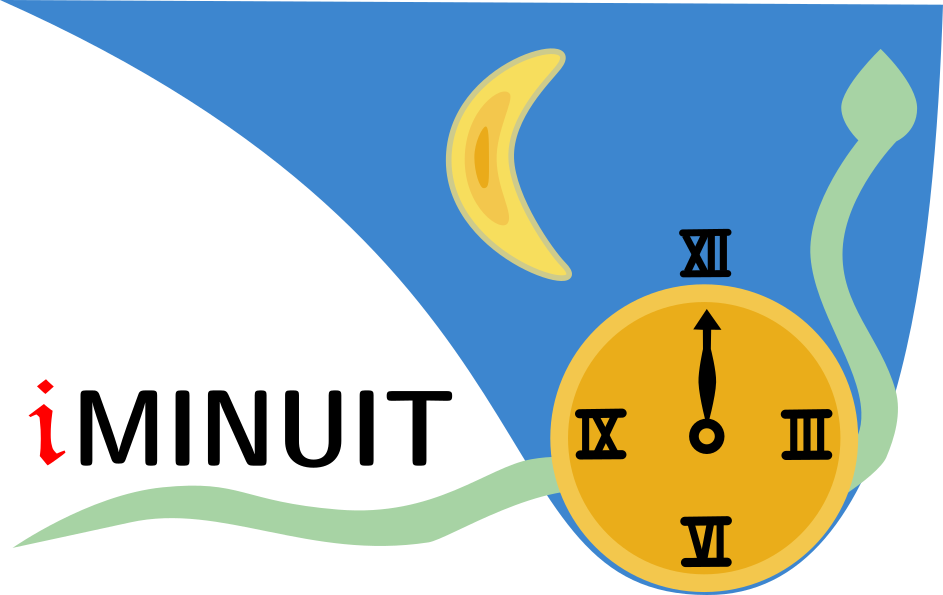
\includegraphics[width=0.8\linewidth]{iminuit-logo.png}

\column{0.8\linewidth}
{\bf iminuit and probfit:} Pythonic interface to Minuit and likelihood builder that works with iminuit.
\end{columns}

\vspace{0.3 cm}
\begin{columns}
\column{2.5 cm}
\column{0.8\linewidth}
{\bf numpythia and pyjet:} interfaces to Pythia and FastJet.
\end{columns}

\vspace{0.3 cm}
\begin{columns}
\column{2.5 cm}
\column{0.8\linewidth}
{\bf decaylanguage, formulate, root\_numpy, vegascope\ldots} packages with focused functionality, broad interfaces.
\end{columns}
\end{frame}

\begin{frame}{uproot}
\hfill \mbox{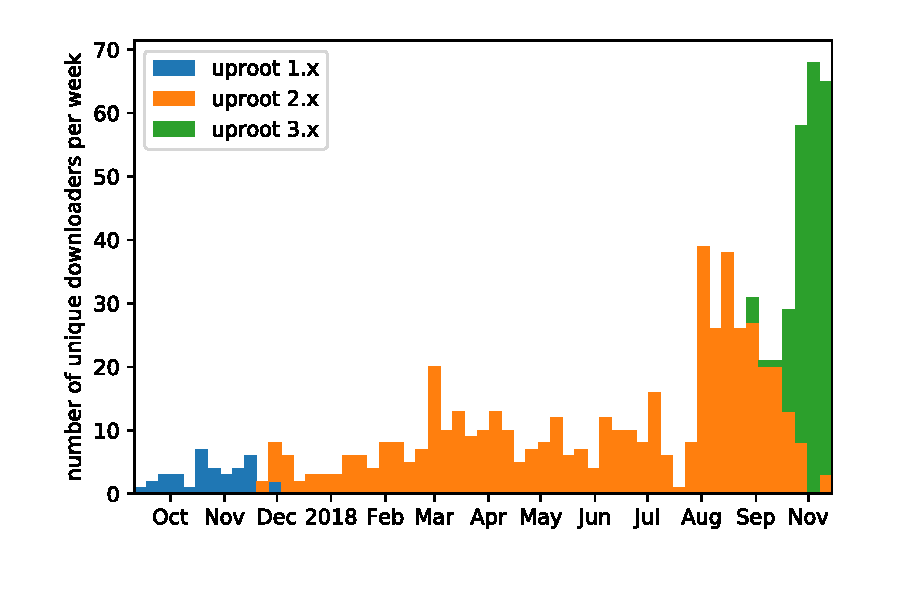
\includegraphics[height=4.5 cm]{weeks_byversion.pdf}\hspace{-1 cm}}

\vspace{-4.25 cm}
Originally, it was a two-week project to access \\ ROOT data in a columnar form more quickly, \\ intended as a backend for a future query service.

\vspace{0.35 cm}
Then I got a lot of feedback from physicists trying \\ to get their data into machine learning libraries.

\vspace{0.35 cm}
So I pivoted, generalized it (2.x), and presented it \\ as an end-user product.

\vspace{0.35 cm}
There are also many users who are just trying to do analysis without ROOT:

\scriptsize
\begin{columns}
\column{0.47\linewidth}
\textcolor{darkgray}{``Great package by the way, the ROOT-independency makes data analysis a lot more flexible.''}

\vspace{0.25 cm}
\textcolor{darkgray}{``Now I'll go through the jagged array tutorial and after that I'll write a wrapper library to make our data accessible without ROOT and any other huge, uncomfortable dependencies, halleluja!''}

\column{0.46\linewidth}

\textcolor{darkgray}{``My particular love of this package is driven by moving away from root as early in my processing as possible and enabling me to use tools I am more comfortable with. I'm not a HEP guy but a space physics guy using geant for instrument responses.''}

\vspace{0.25 cm}
\textcolor{darkgray}{``Thank you for all of your work with this, being able to load root files without ROOT is wonderful!''}
\end{columns}
\end{frame}

%% ``So, in my case, the arrays function are equivalent to numpy load to native format. Very impressive!!! Kudos!!!''

%% ``Also, I'm very excited to see what you do with jagged arrays. They caused me a lot of problems when I started my work with numpy several years ago. I'm happy to know someone is formalizing a way for them to play well with numpy. thanks again for all your work!''

\begin{frame}{uproot implementation philosophy}
\vspace{0.4 cm}
Based on the observation that:
\begin{itemize}
\item a Numpy analysis operates on one column of data at a time, and
\item data in a ROOT file are already arranged in columns.
\end{itemize}

\vspace{0.25 cm}
Transforming columnar bytes on disk into event records back into columnar arrays is undesirable extra work. Dropping it makes up for seeking to the positions of the columnar arrays using slow Python, {\it if the arrays (baskets) are large.}

\begin{columns}
\column{0.5\linewidth}
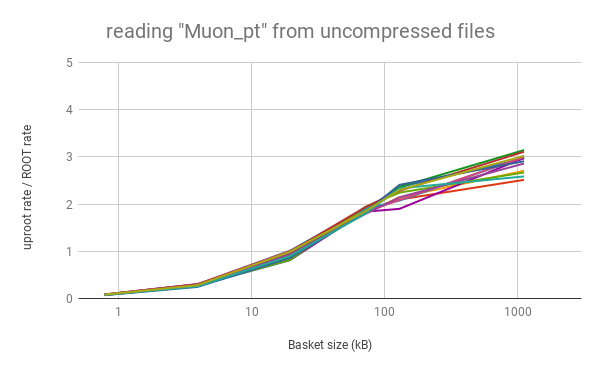
\includegraphics[width=\linewidth]{root-none-muon.png}

\column{0.5\linewidth}
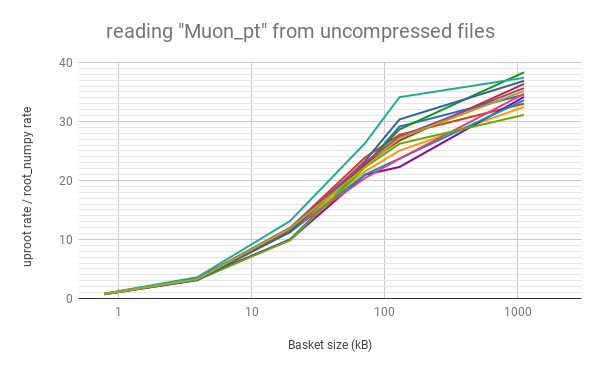
\includegraphics[width=\linewidth]{rootnumpy-none-muon.png}
\end{columns}
\end{frame}

\begin{frame}{uproot dependencies}
\vspace{0.5 cm}
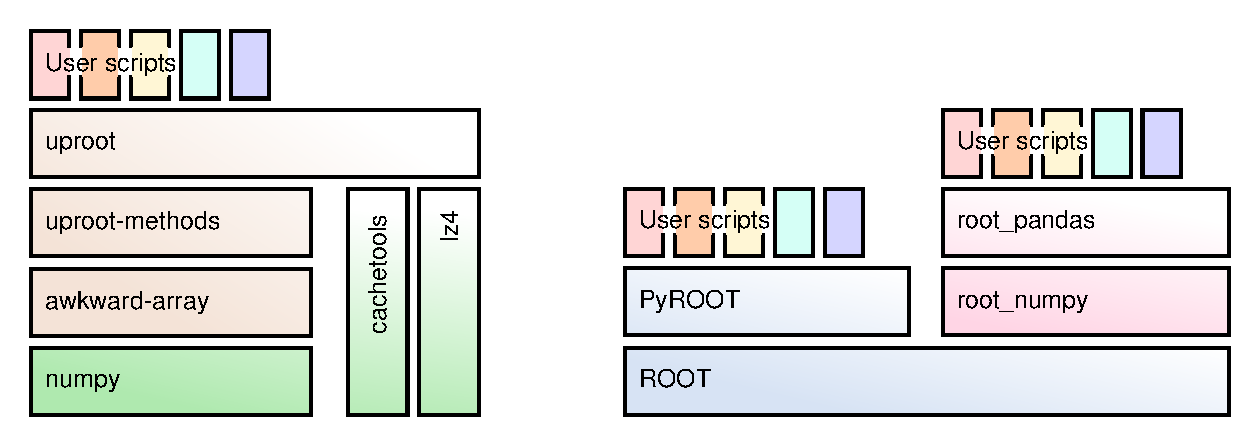
\includegraphics[width=\linewidth]{abstraction-layers.pdf}

\vspace{0.5 cm}
Pythonic interfaces to objects extracted from ROOT (e.g.\ histograms, Lorentz vectors) have been moved to uproot-methods, to evolve on a different schedule and accept more user-contributed pull requests.
\end{frame}

\begin{frame}[fragile]{uproot example}
\small
\vspace{0.1 cm}
\begin{columns}
\column{1.1\linewidth}
\begin{minted}{python}
>>> import uproot
>>> tree = uproot.open("HZZ-objects.root")["events"]   # dict-like
>>> array = tree.array("muonp4")

>>> array                                # all events
<JaggedArray [[TLorentzVector(-52.899, -11.655, -8.1608, 54.779)
               TLorentzVector(37.738, 0.69347, -11.308, 39.402)] ...]>
>>> array[0][1]                          # second particle in first event
TLorentzVector(37.738, 0.69347, -11.308, 39.402)

>>> hastwo = (array.counts >= 2)         # events with at least two muons
>>> leading = array[hastwo, 0]           # mask and select first
>>> subleading = array[hastwo, 1]        # mask and select second

>>> candidates = leading + subleading    # Lorentz vector sum across all
>>> candidates.mass                      # compute mass for all
array([90.22779777, 74.74654928, ..., 85.44384208, 75.96066262])
\end{minted}
\end{columns}
\end{frame}



\end{document}
